\documentclass[mathserif,compress]{beamer}\usepackage{graphicx, color}
%% maxwidth is the original width if it is less than linewidth
%% otherwise use linewidth (to make sure the graphics do not exceed the margin)
\makeatletter
\def\maxwidth{ %
  \ifdim\Gin@nat@width>\linewidth
    \linewidth
  \else
    \Gin@nat@width
  \fi
}
\makeatother

\definecolor{fgcolor}{rgb}{0.2, 0.2, 0.2}
\newcommand{\hlnumber}[1]{\textcolor[rgb]{0,0,0}{#1}}%
\newcommand{\hlfunctioncall}[1]{\textcolor[rgb]{0.501960784313725,0,0.329411764705882}{\textbf{#1}}}%
\newcommand{\hlstring}[1]{\textcolor[rgb]{0.6,0.6,1}{#1}}%
\newcommand{\hlkeyword}[1]{\textcolor[rgb]{0,0,0}{\textbf{#1}}}%
\newcommand{\hlargument}[1]{\textcolor[rgb]{0.690196078431373,0.250980392156863,0.0196078431372549}{#1}}%
\newcommand{\hlcomment}[1]{\textcolor[rgb]{0.180392156862745,0.6,0.341176470588235}{#1}}%
\newcommand{\hlroxygencomment}[1]{\textcolor[rgb]{0.43921568627451,0.47843137254902,0.701960784313725}{#1}}%
\newcommand{\hlformalargs}[1]{\textcolor[rgb]{0.690196078431373,0.250980392156863,0.0196078431372549}{#1}}%
\newcommand{\hleqformalargs}[1]{\textcolor[rgb]{0.690196078431373,0.250980392156863,0.0196078431372549}{#1}}%
\newcommand{\hlassignement}[1]{\textcolor[rgb]{0,0,0}{\textbf{#1}}}%
\newcommand{\hlpackage}[1]{\textcolor[rgb]{0.588235294117647,0.709803921568627,0.145098039215686}{#1}}%
\newcommand{\hlslot}[1]{\textit{#1}}%
\newcommand{\hlsymbol}[1]{\textcolor[rgb]{0,0,0}{#1}}%
\newcommand{\hlprompt}[1]{\textcolor[rgb]{0.2,0.2,0.2}{#1}}%

\usepackage{framed}
\makeatletter
\newenvironment{kframe}{%
 \def\at@end@of@kframe{}%
 \ifinner\ifhmode%
  \def\at@end@of@kframe{\end{minipage}}%
  \begin{minipage}{\columnwidth}%
 \fi\fi%
 \def\FrameCommand##1{\hskip\@totalleftmargin \hskip-\fboxsep
 \colorbox{shadecolor}{##1}\hskip-\fboxsep
     % There is no \\@totalrightmargin, so:
     \hskip-\linewidth \hskip-\@totalleftmargin \hskip\columnwidth}%
 \MakeFramed {\advance\hsize-\width
   \@totalleftmargin\z@ \linewidth\hsize
   \@setminipage}}%
 {\par\unskip\endMakeFramed%
 \at@end@of@kframe}
\makeatother

\definecolor{shadecolor}{rgb}{.97, .97, .97}
\definecolor{messagecolor}{rgb}{0, 0, 0}
\definecolor{warningcolor}{rgb}{1, 0, 1}
\definecolor{errorcolor}{rgb}{1, 0, 0}
\newenvironment{knitrout}{}{} % an empty environment to be redefined in TeX

\usepackage{alltt} 
\usepackage{beamerthemeDresden} 
\usepackage[english]{babel}
\usepackage{amsmath,amssymb}
\usepackage[latin1]{inputenc}
\usepackage{palatino}
\usepackage{graphicx}
\usepackage{subfigure}
\usepackage{pgf}
\usepackage{relsize}
\def\beq{\begin{equation}}
\def\eeq{\end{equation}}
\def\bit{\begin{itemize}}
\def\eit{\end{itemize}}
\def\bdm{\begin{displaymath}}
\def\edm{\end{displaymath}}
\def\ben{\begin{enumerate}}
\def\een{\end{enumerate}}
\def\bb{\mathbf{b}}
\def\bc{\mathbf{c}}
\def\bd{\mathbf{d}}
\def\bh{\mathbf{h}}
\def\bm{\mathbf{m}}
\def\br{\mathbf{r}}
\def\bs{\mathbf{s}}
\def\bu{\mathbf{u}}
\def\bv{\mathbf{v}}
\def\bw{\mathbf{w}}
\def\bx{\mathbf{x}}
\def\by{\mathbf{y}}
\def\bz{\mathbf{z}}
\def\bA{\mathbf{A}}
\def\bD{\mathbf{D}}
\def\bG{\mathbf{G}}
\def\bI{\mathbf{I}}
\def\bQ{\mathbf{Q}}
\def\bR{\mathbf{R}}
\def\bS{\mathbf{S}}
\def\bV{\mathbf{V}}
\def\bW{\mathbf{W}}
\def\bX{\mathbf{X}}
\def\bY{\mathbf{Y}}
\def\bZ{\mathbf{Z}}
\def\cB{\mathcal{B}}
\def\cF{\mathcal{F}}
\def\cI{\mathcal{I}}
\def\cK{\mathcal{K}}
\def\cU{\mathcal{U}}
\def\bbeta{\mbox{\boldmath $\beta$}}
\def\bepsilon{\mbox{\boldmath $\epsilon$}}
\def\bdelta{\mbox{\boldmath $\delta$}}
\def\bgamma{\mbox{\boldmath $\gamma$}}
\def\bldeta{\mbox{\boldmath $\eta$}}
\def\bphi{\mbox{\boldmath $\phi$}}
\def\bkappa{\mbox{\boldmath $\kappa$}}
\def\blambda{\mbox{\boldmath $\lambda$}}
\def\bmu{\mbox{\boldmath $\mu$}}
\def\bnu{\mbox{\boldmath $\nu$}}
\def\btheta{\mbox{\boldmath $\theta$}}
\def\brho{\mbox{\boldmath $\rho$}}
\def\bDelta{\mbox{\boldmath $\Delta$}}
\def\bLambda{\mbox{\boldmath $\Lambda$}}
\def\bSigma{\mbox{\boldmath $\Sigma$}}
\def\var{\textrm{var}}
\def\cov{\textrm{cov}}
\def\log{\textrm{log}}
\def\median{\textrm{median}}
\def\argmin{\textrm{arg min }}
\def\bzero{\mathbf{0}}
\def\bone{\mathbf{1}}
\def\Poi{\textrm{Poi}}
\def\Unif{\textrm{Unif}}
\def\upp{^\prime}
\def\upi{^{-1}}
\newcommand{\cye}[1]{\color{yellow!70!black}#1}
\newcommand{\cre}[1]{\color{red!70!black}#1}
\newcommand{\cbl}[1]{\color{blue!70!black}#1}
\newcommand{\cgr}[1]{\color{green!70!black}#1}
\newcommand{\cS}{\ensuremath{\mathcal{S}}}
\IfFileExists{upquote.sty}{\usepackage{upquote}}{}

\begin{document}


\title[]{Estimating Abundance from Counts in Large Data Sets of Irregularly-Spaced Plots using Spatial Basis Functions}

\author[Jay M. Ver Hoef]{Jay Ver Hoef} 

\institute[NOAA National Marine Mammal Lab]
{
	\normalsize NOAA National Marine Mammal Lab \\
	NOAA Fisheries \\
	International Arctic Research Center \\
	Fairbanks, Alaska, USA\\
	\vspace{0.1cm}
}
\date[05/17/13]{}
 
\maketitle
 
% very important to use option [fragile] for frames containing code output!
%-------------------------------------------------------------------------------
%                        Introduction
%-------------------------------------------------------------------------------

\section{Introduction}
\subsection{}
\begin{frame}[fragile]
\frametitle{Introduction}
	
	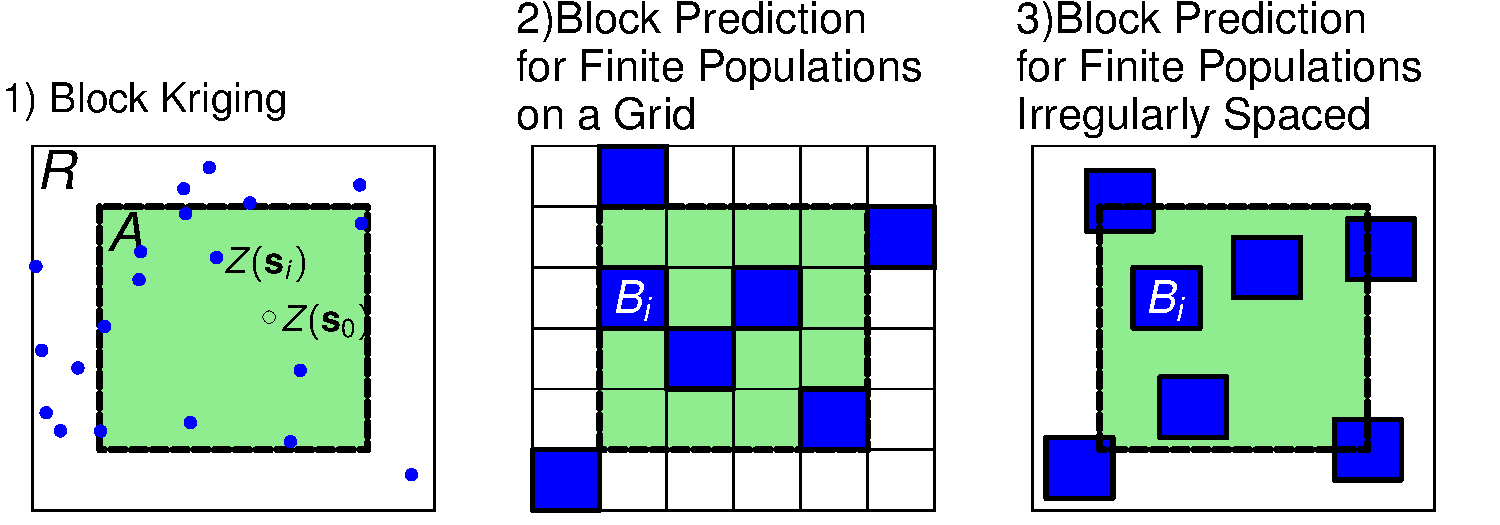
\includegraphics[width=\maxwidth]{figure/Introductory-plot}

\vspace{.5cm}
\scriptsize

\end{frame}

%-------------------------------------------------------------------------------
%                        Motivating Example
%-------------------------------------------------------------------------------

\begin{frame}[fragile]
\frametitle{Motivating Example}




\vspace{-1cm}
\begin{center}
	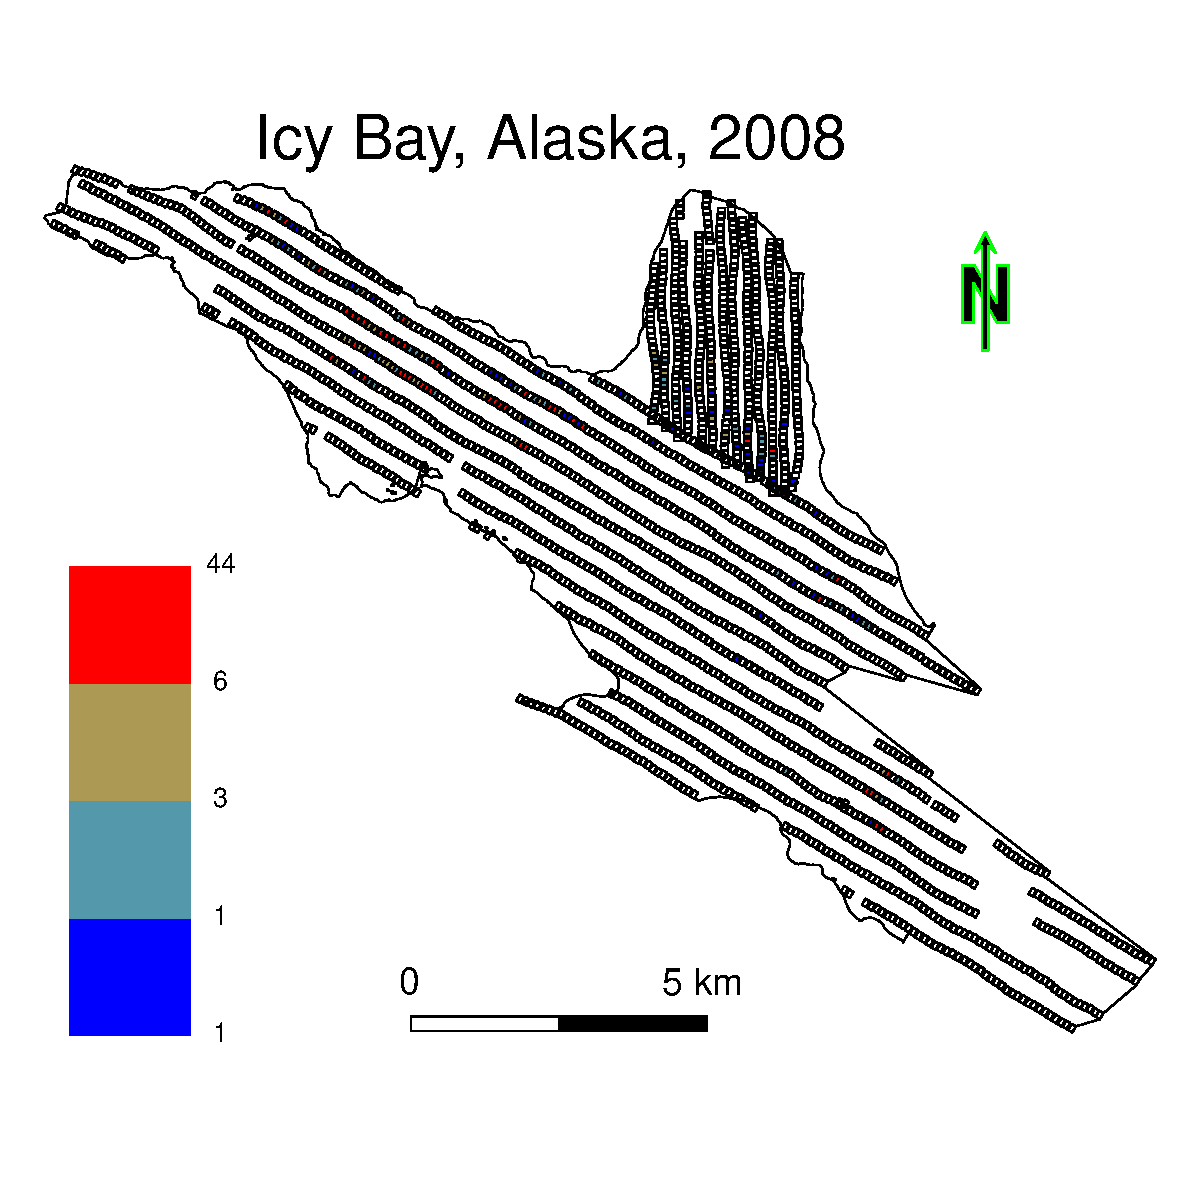
\includegraphics[width = .8\maxwidth]{figure/icyBayIntro-plot} 
\end{center}

\end{frame}

%-------------------------------------------------------------------------------
%                        Goals
%-------------------------------------------------------------------------------

\begin{frame}[fragile]
\frametitle{Goals}

\footnotesize
	An estimator that is:
		\begin{itemize}
		\item fast to compute, robust, and requires few modeling decisions, similar to classical survey methods, 			\item based only on counts within plots; actual spatial locations of animals are unknown, 
		\item for the actual number of seals, not the mean of some assumed process that generated the data, 
		\item have a variance estimator with a population correction factor that shrinks to zero as the proportion of the study area that gets sampled goes to one, 
		\item unbiased with valid confidence intervals, 
		\item able to accommodate nonstationary variance and excessive zeros throughout the area
		\end{itemize}

\end{frame}

%-------------------------------------------------------------------------------
%                       Inhomogeneous Spatial Point Processes
%-------------------------------------------------------------------------------

\section{Model}
\subsection{}
\begin{frame}[fragile]
\frametitle{Inhomogeneous Spatial Point Processes}

	$T(V)$ is the total number of points in planar region $V$
	\begin{center}
		$\lambda(\bs) = \lim_{|dx| \to 0} \frac{E\left( T(dx) \right) }{|dx|}$ \\
	\end{center}
	{\em Expected} abundance in $A \subseteq R$: \\
	\begin{center}
		$\mu(A)=\int_A \lambda(\bu|\btheta)d\bu$ \\
	\end{center}
	Abundance is assumed random \\
	\begin{center}
		$T(A) \sim \Poi(\mu(A))$ \\
	\end{center}
	Resulting in an observed pattern $\cS^+ = (\bs_1,\dots,\bs_N)$

\end{frame}

%-------------------------------------------------------------------------------
%                       Outline of an Estimator
%-------------------------------------------------------------------------------

\begin{frame}[fragile]
\frametitle{Outline of an Estimator}




	\begin{tabular}{p{4.0cm} p{5.5cm}}
		\vspace{.1cm}
		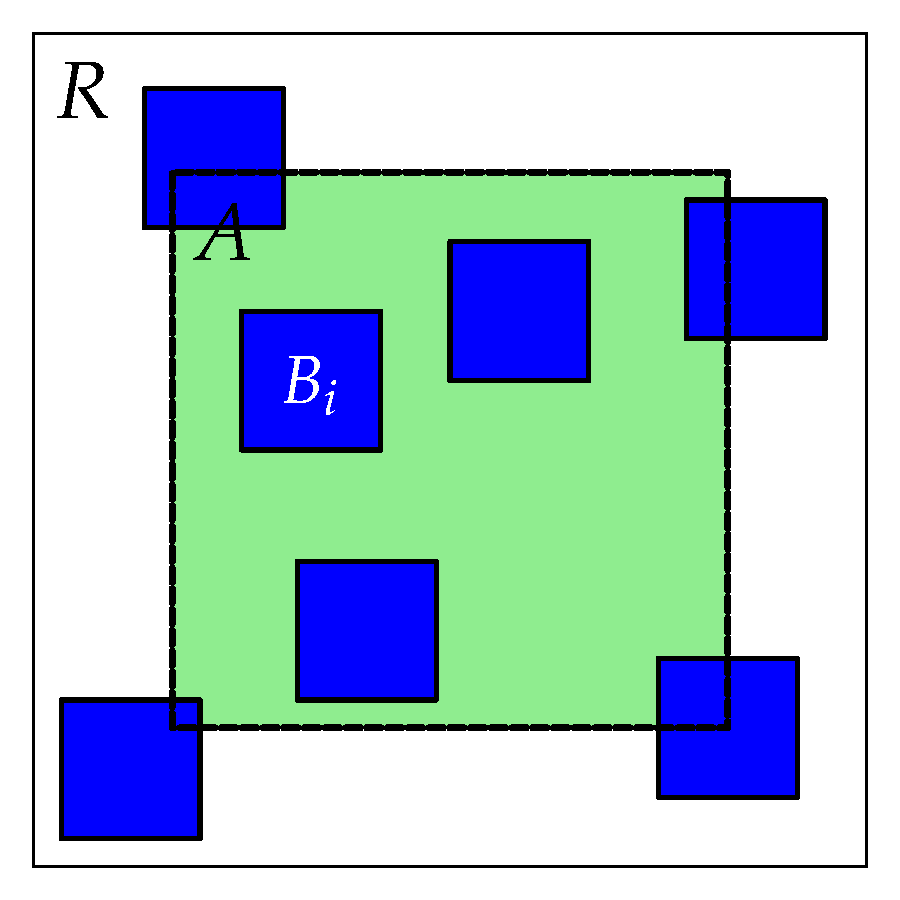
\includegraphics[width = \maxwidth]{figure/irregSamples-plot} &
		\vspace{-.1cm}
		\begin{itemize}
			\item $\cB = \cup_{i = 1}^n (B_i \cap A)$
			\item $\cU \equiv \overline{\cB} \cap A$
			\item $T(A) = T(\cB) + T(\cU)$
			\item $T(\cU) \sim \Poi(\mu(\cU))$
			\item $\mu(\cU)= \int_{\cU} \lambda(\bu|\btheta) d\bu$
			\item $\widehat{T}(A) = T(\cB) + \widehat{T}(\cU)$
			\footnotesize
			\item $T(\cB) \rightarrow T(A) \Rightarrow \widehat{T}(A) \rightarrow T(A)$
		\end{itemize}
	\end{tabular}

\end{frame}

%-------------------------------------------------------------------------------
%                    From IPP to Poisson Regression
%-------------------------------------------------------------------------------

\begin{frame}[fragile]
\frametitle{From IPP to Poisson Regression}

	\begin{tabular}{p{3.5cm} p{7.0cm}}
		\vspace{.1cm}
		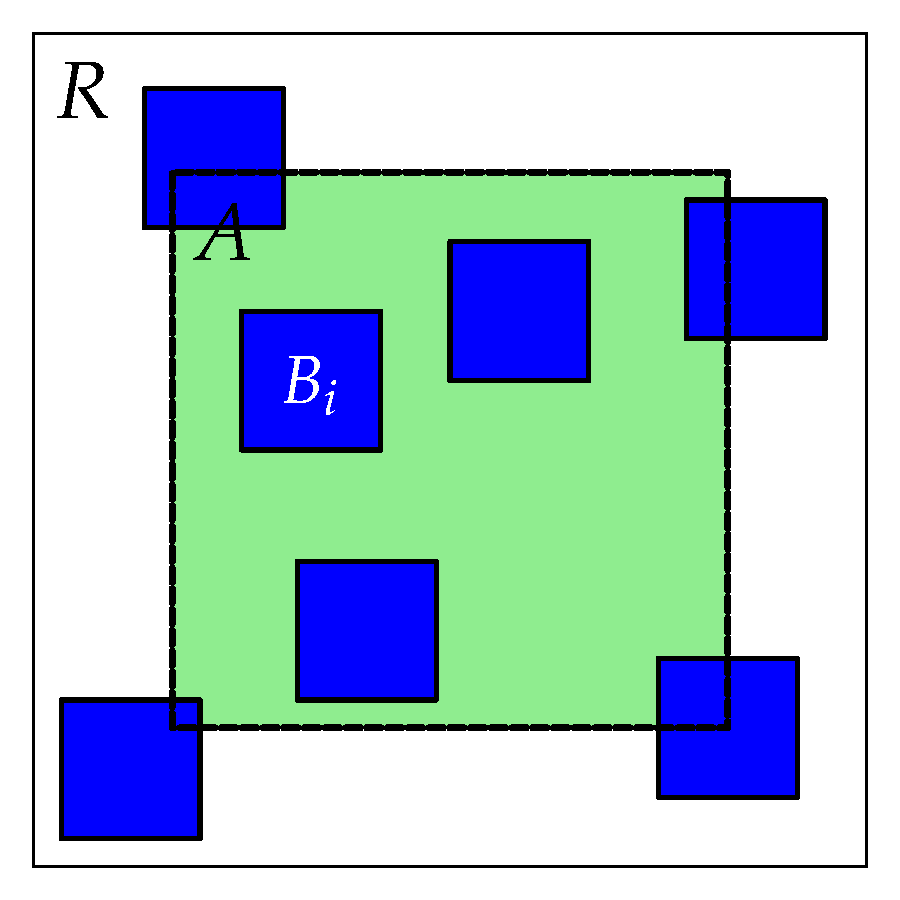
\includegraphics[width = \maxwidth]{figure/irregSamples-plot} &
		\vspace{-.1cm}
		\begin{itemize}
			\item $Y(B_i) \sim \Poi(\mu(B_i))$
			\item $\mu(B_i) = \int_{B_i}\lambda(\bu|\btheta) d\bu$
			\item Let $\bs_i$ be centroid of $B_i$
			\item $\mu(B_i) \approx |{B_i}|\lambda(\bs_i|\btheta)$
			\item $\log(\mu(B_i)) = \log(|B_i|) + \log(\lambda(\bs_i|\btheta))$
			\item $\log(\lambda(\bs_i|\btheta)) = \bx(\bs_i)^\prime\bbeta$
		\end{itemize}
	\end{tabular}
Now us spatial basis functions to generate $\bx(\bs_i)$

\end{frame}

%-------------------------------------------------------------------------------
%                    Spatial Basis Functions
%-------------------------------------------------------------------------------

\begin{frame}[fragile]
\frametitle{Spatial Basis Functions}




	\begin{tabular}{p{5.0cm} p{5.5cm}}
		\vspace{.1cm}
		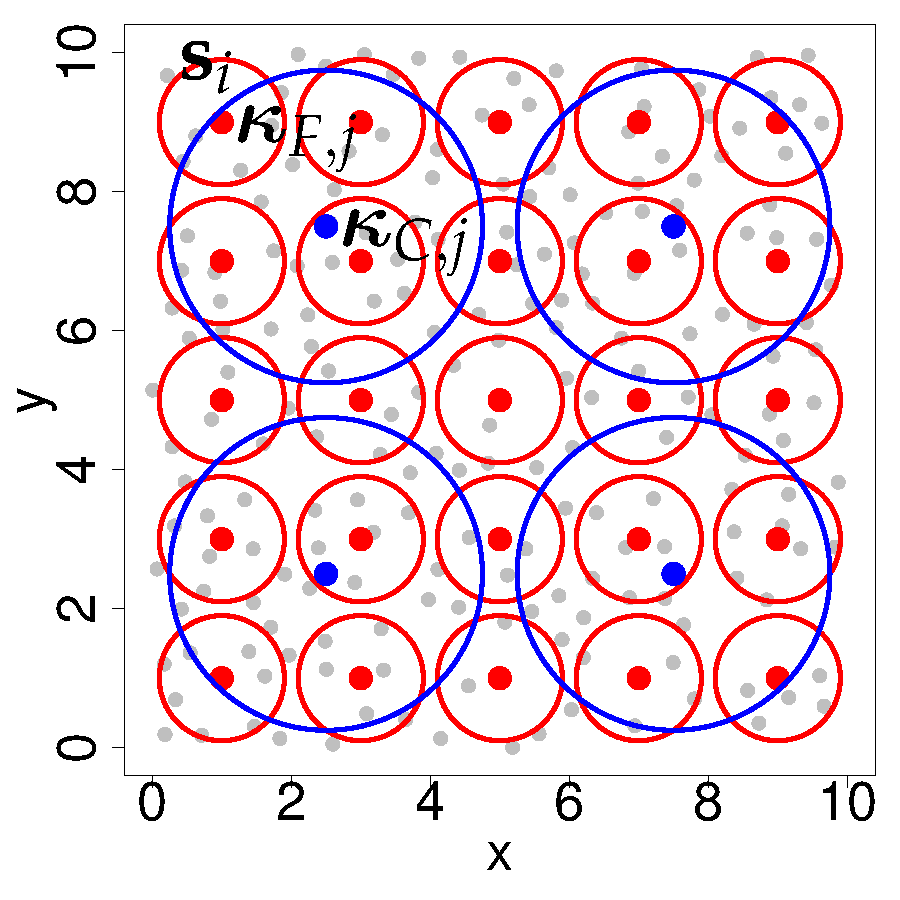
\includegraphics[width = 5.5cm]{figure/spatialBasisExplanation-plot} &
		\vspace{1cm}
		\begin{itemize}
			\item $C(h;\rho)=\exp(-h^2/\rho)$
			\item $\bX_{i,j} = C(\| \bs_i-\bkappa_{F,j})\|;\rho_F);$ \footnotesize $j = 2,\ldots,K_F + 1$
			\item $\bX_{i,j} = \normalsize C(\| \bs_i-\bkappa_{C,j})\|;\rho_C);$ \footnotesize $j = K_F + 2,\ldots,K_F + K_C + 1$
		\end{itemize}
	\end{tabular}
\footnotesize
knot location: k-means clustering of dense grid of spatial coordinates

\end{frame}

%-------------------------------------------------------------------------------
%                    Fitting the Model
%-------------------------------------------------------------------------------

\begin{frame}[fragile]
\frametitle{Fitting the Model}

minimize minus the log-likelihood:
\begin{center}
	$-\ell(\brho,\bbeta;\by) \propto \sum_{i=1}^{n} |B_i|\exp(\bx_{\brho}(\bs_i)\upp\bbeta) - y_i\log|B_i| - y_i\bx_{\brho}(\bs_i)\upp\bbeta$
\end{center}
Two-part algorithm: 
\begin{itemize}
	\item Condition on $\brho$ and use IWLS to estimate $\bbeta$ (with offset for $|B_i|$, ala GLMs)
	\item optimize for $\brho$ numerically
\end{itemize}

\end{frame}

%-------------------------------------------------------------------------------
%                    Back to the Estimator
%-------------------------------------------------------------------------------

\section{Inference}
\subsection{}
\begin{frame}[fragile]
\frametitle{Back to the Estimator}

\begin{itemize}
	\item $\widehat{T}(A) = T(\cB) + \widehat{T}(\cU)$
	\item $\widehat{T}(\cU) =\mu(\cU)=\int_\cU \lambda(\bu|\hat{\brho},\hat{\bbeta})d\bu$
	\item $ \lambda(\bu|\hat{\brho},\hat{\bbeta}) = \exp(\bx_{\hat{\brho}}(\bu)\upp\hat{\bbeta})$
\end{itemize}
Approximate integral with dense grid of $n_p$ points within $\bu_j \in \cU$.
\begin{center}
$\widehat{T}(A) = T(\cB) + \sum_{j=1}^{n_p}|U_i|\exp(\bx_{\hat{\brho}}(\bu_j)\upp\hat{\bbeta})$
\end{center}
where $|U_i|$ is a small area around each $\bu_j$
\end{frame}

%-------------------------------------------------------------------------------
%                    Variance
%-------------------------------------------------------------------------------

\begin{frame}[fragile]
\frametitle{Variance}

$\textrm{MSPE}(\hat{T}(A)) = E[(\hat{T}(A) - T(A))^2;\bbeta] = E[(\hat{T}(\cU) - T(\cU))^2;\bbeta]$
Note: as $\cU \cap A \to \varnothing \Rightarrow \textrm{MSPE}(\widehat{T}(A)) \to 0$ \\
From IPP assumption: $\hat{T}(\cU)$ independent from $T(\cU)$. \\
Assuming unbiasedness, $E[(\hat{T}(\cU)] = E[T(\cU)]$,
\begin{center}
$\textrm{MSPE} = \var[T(\cU);\bbeta] + \var[\hat{T}(\cU);\bbeta]$ \\
$= \mu(\cU;\bbeta) + \var[\hat{T}(\cU);\bbeta]$ \\
\end{center}
Now, what about $\var[\hat{T}(\cU);\bbeta]$?
\end{frame}

%-------------------------------------------------------------------------------
%                    Variance
%-------------------------------------------------------------------------------

\begin{frame}[fragile]
\frametitle{Variance}

Recall delta method result: $\var(f(\by)) \approx \bd\upp\bSigma\bd$ \\
\tiny
Jay M. Ver Hoef (2012) Who Invented the Delta Method? The American Statistician, 66:2, 124-127 \\
\normalsize
where $\var(\by) = \bSigma$ and $d_i = \partial f(\by)/\partial y_i$ \\
\footnotesize
\[
	d_i = \frac{\partial \hat{T}(\cU)}{\partial \beta_i} = \int_{\cU}x_i(\bu)\exp(\bx(\bu)^\prime\hat{\bbeta}) d\bu \approx \frac{|\cU|}{n_p}\sum_{i=1}^{n_p} x_i(\bs_i)\exp(\bx(\bs_i)^\prime\hat{\bbeta})
\]
\normalsize
From Rathbun and Cressie, (1994), if $\hat{\bbeta}$ is MLE,
\footnotesize
\[
\hat{\bSigma}= \left[\sum_{i=1}^n\int_{B_i} \bx(\bs)\bx({\bs})\upp\exp(\bx(\bs)\upp \hat{\bbeta}) d\bs\right]\upi \approx \left[ |B| \sum_{i=1}^{n} \bx(\bs_i)\bx({\bs_i})\upp\exp(\bx(\bs_i)\upp \hat{\bbeta}) \right]\upi
\]
\normalsize
if $|B_i| = |B| \ \forall \ i$. \\
\vspace{.2cm}
\tiny
Rathbun, S. L. and Cressie, N. (1994), ``Asymptotic Properties of Estimators for the Parameters of Spatial Inhomogeneous Poisson Point Processes,'' Advances in Applied Probability, 26, 122-154.

\end{frame}

%-------------------------------------------------------------------------------
%                    Summary
%-------------------------------------------------------------------------------

\begin{frame}[fragile]
\frametitle{Summary}

\begin{center}
$\widehat{T}(A) = T(\cB) + \frac{|\cU|}{n_p}\sum_{j=1}^{n_p}\exp(\bx_{\hat{\brho}}(\bu_j)\upp\hat{\bbeta})$
\end{center} 
\begin{center}
\[
\begin{array}{rl}
\widetilde{\var}(\widehat{T}(A)) = & \frac{|\cU|}{n_p}\sum_{j=1}^{n_p}\exp(\bx_{\hat{\brho}}(\bu_j)\upp\hat{\bbeta}) + \\ & \bd\upp\left[ |B| \sum_{i=1}^{n} \bx(\bs_i)\bx({\bs_i})\upp\exp(\bx(\bs_i)\upp \hat{\bbeta}) \right]\upi\bd
\end{array}
\]
\end{center} 
where \\
\begin{center}
 $d_i = \frac{|\cU|}{n_p}\sum_{i=1}^{n_p} x_i(\bs_i)\exp(\bx(\bs_i)^\prime\hat{\bbeta})$
\end{center}

\end{frame}

%-------------------------------------------------------------------------------
%                    Overdispersion
%-------------------------------------------------------------------------------

\begin{frame}[fragile]
\frametitle{Simulated Example}




	\vspace{-.1cm}
	\begin{center}
	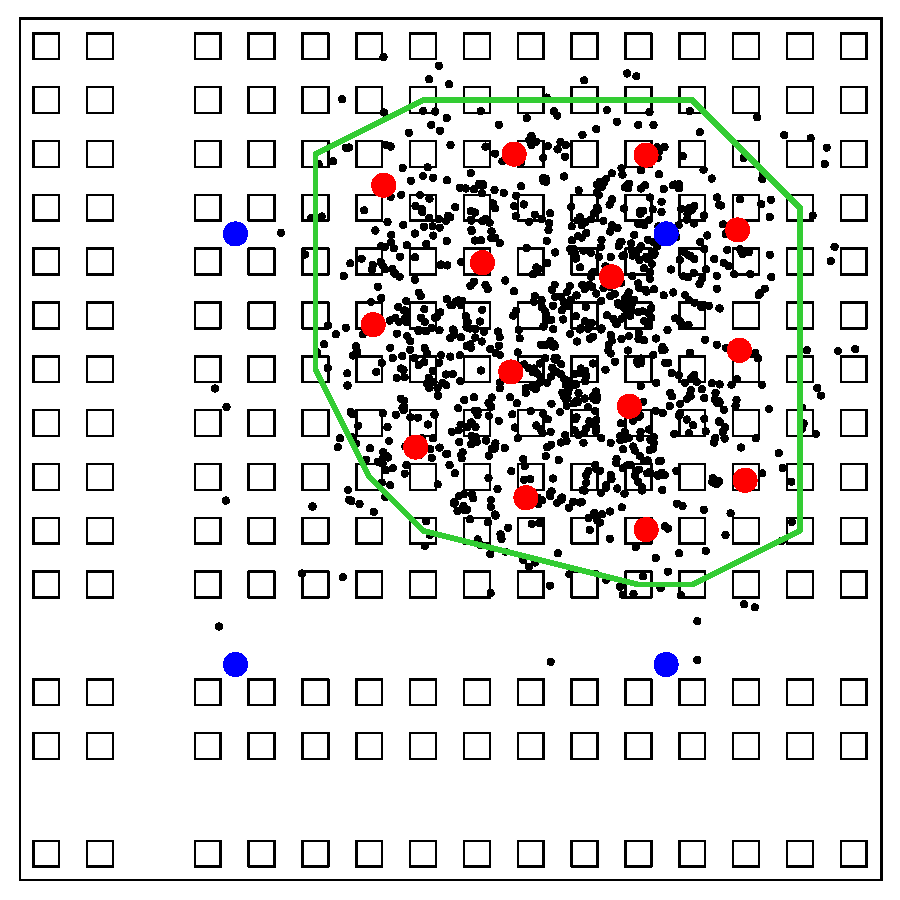
\includegraphics[width = .6\maxwidth]{figure/sim2-plot}
	\end{center}

\end{frame}

\begin{frame}[fragile]
\frametitle{Simulated Example}




		\vspace{-.1cm}
		\begin{center}
		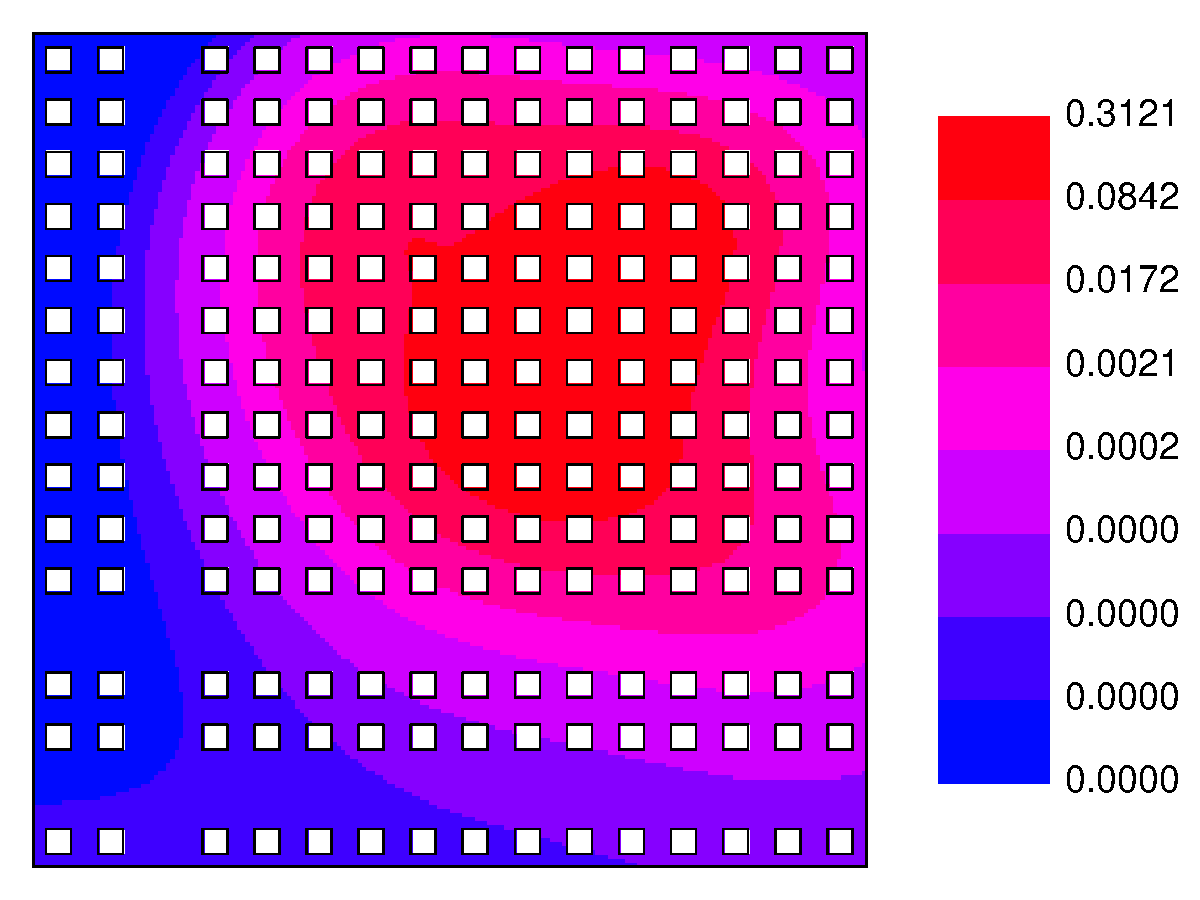
\includegraphics[width = .55\maxwidth]{figure/exFittedSurface-plot} \\
		\end{center}
		\vspace{-.2cm}
		True abundance was 1079 \\
		Estimated abundance was 1143 with standard error 62

\end{frame}

%-------------------------------------------------------------------------------
%                    Overdispersion
%-------------------------------------------------------------------------------

\section{Overdispersion}
\subsection{}
\begin{frame}[fragile]
\frametitle{Residuals Plots}







	\vspace{-.1cm}
	\begin{center}
	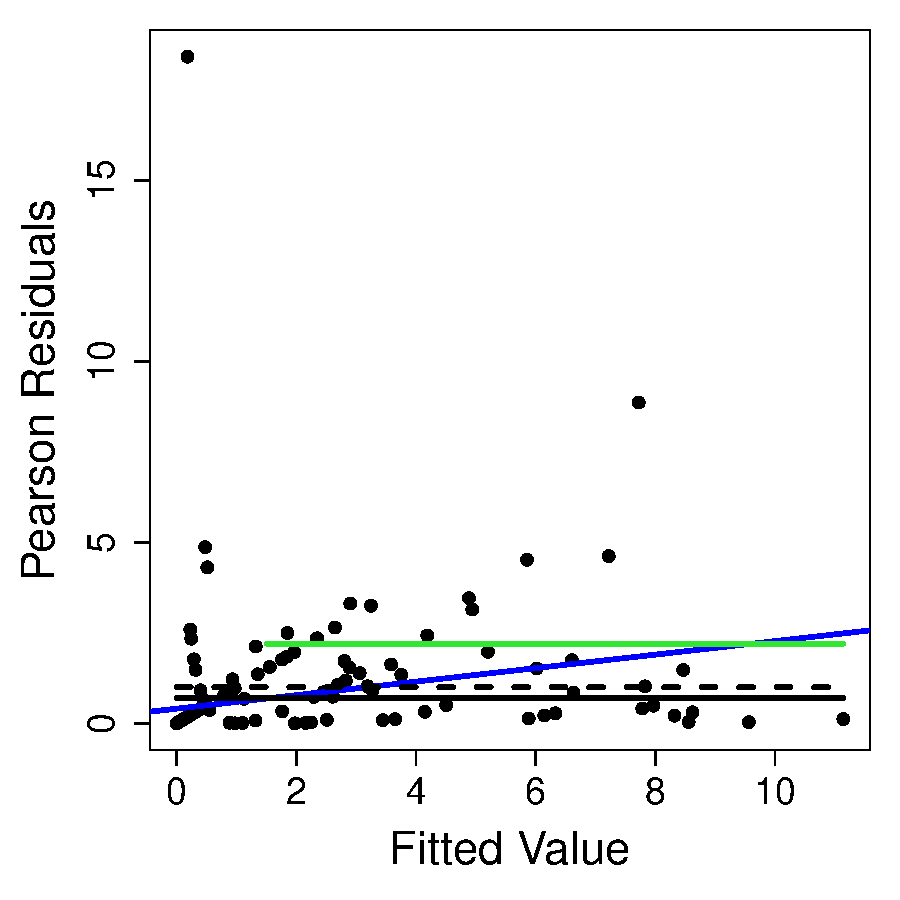
\includegraphics[width = .5\maxwidth]{figure/resids4overdisp-plot}
	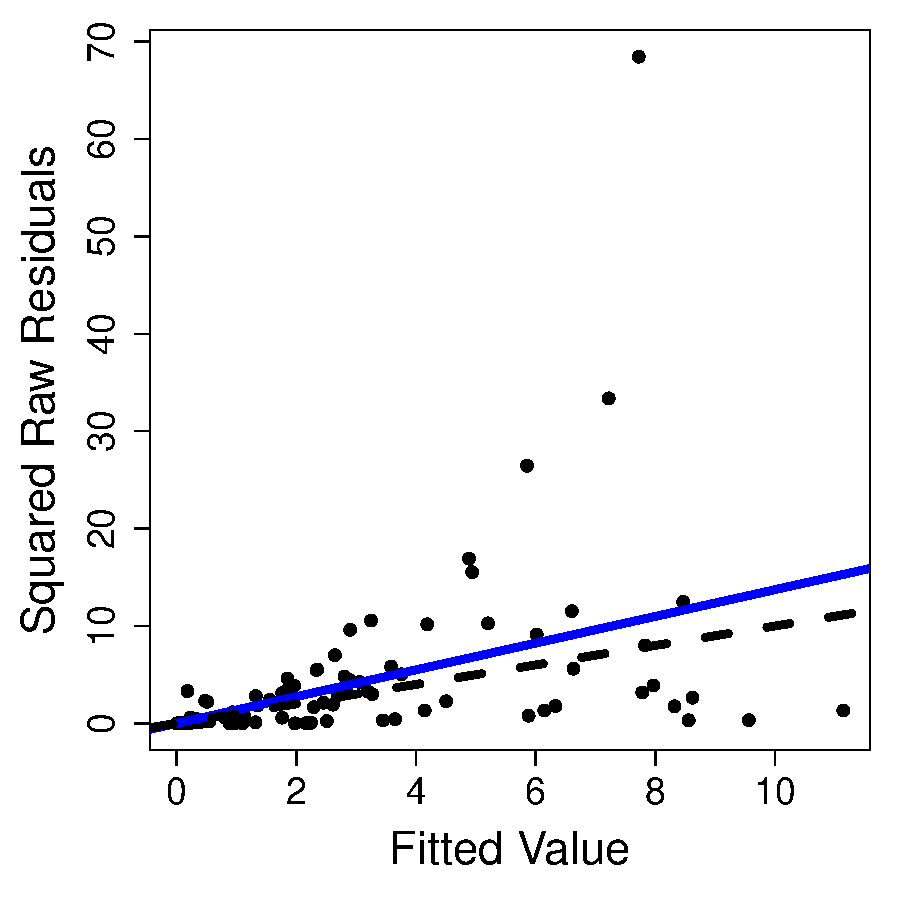
\includegraphics[width = .5\maxwidth]{figure/rawresids4overdisp-plot}
	\end{center}

\end{frame}

%-------------------------------------------------------------------------------
%                    Overdispersion Estimators
%-------------------------------------------------------------------------------

\begin{frame}[fragile]
\frametitle{Overdispersion Estimators}

	\begin{itemize}
	\item The traditional estimator:
	\[
	\omega_{OD} = \max\left(1, \frac{1}{n-r}\sum_{i=1}^n\frac{(y_i-\phi_i)^2}{\phi_i}\right)
	\]
	where $r$ is the rank of $\bX$.
	\item Weighted regression estimator:
	\[
	\omega_{WR} = \max\left(1, \arg\underset{\omega}{\min}\sum_{i=1}^n\sqrt{\phi_i}[(y_i - \phi_i)^2 - \omega\phi_i]^2\right),
	\]
	where $\sqrt{\phi_i}$ were the weights
	\end{itemize}

\end{frame}

%-------------------------------------------------------------------------------
%                    Overdispersion Estimators
%-------------------------------------------------------------------------------

\begin{frame}[fragile]
\frametitle{Overdispersion Estimators}

	\begin{itemize}
	\item Trimmed Mean:
	\[
	\omega_{TG}(p) = \max\left(1, \frac{1}{n - \lfloor np \rfloor -r}
		\sum_{i = \lfloor np \rfloor + 1}^n\frac{(y_{(i)}-\phi_{(i)})^2}{\phi_{(i)}}\right)
	\]
	where $0 \le p \le 1$, $y_{(i)}$ and $\phi_{(i)}$ are ordered values, and $\lfloor x \rfloor$ rounds $x$ down to the nearest integer.
	\end{itemize}

\end{frame}

%-------------------------------------------------------------------------------
%                    Adjusted Variance Estimators
%-------------------------------------------------------------------------------

\begin{frame}[fragile]
\frametitle{Adjusted Variance Estimators}

	\begin{itemize}
	\item 
	$\widehat{\var}_{OD}(\widehat{T}(A)) = \omega_{OD}\widetilde{\var}(\widehat{T}(A))$
	\item 
	$\widehat{\var}_{WR}(\widehat{T}(A)) = \omega_{WR}\widetilde{\var}(\widehat{T}(A))$
	\item 
	$\widehat{\var}_{TG}(\widehat{T}(A);p) = \omega_{TG}(p)\widetilde{\var}(\widehat{T}(A))$
	\item 
$\widehat{\var}_{TL}(\widehat{T}(A);p) = \frac{|\cU|}{n_p}\sum_{j=1}^{n_p}\exp(\bx_{\hat{\brho}}(\bu_j)\upp\hat{\bbeta})\times$ $\max(1,\omega_{TG}(p)I(\exp(\bx(\bs_j)\upp \hat{\bbeta}) \ge \phi_{(\lfloor np \rfloor)}) + $  $\bd\upp\left[ |B| \sum_{i=1}^{n} \bx(\bs_i)\bx({\bs_i})\upp\exp(\bx(\bs_i)\upp \hat{\bbeta}) \right]\upi\bd $ \\
where $I(\cdot)$ is the indicator function
	\end{itemize}

\end{frame}

%-------------------------------------------------------------------------------
%                    Simulations
%-------------------------------------------------------------------------------

\section{Simulations}
\subsection{}
\begin{frame}[fragile]
\frametitle{Simulations}

\begin{center}
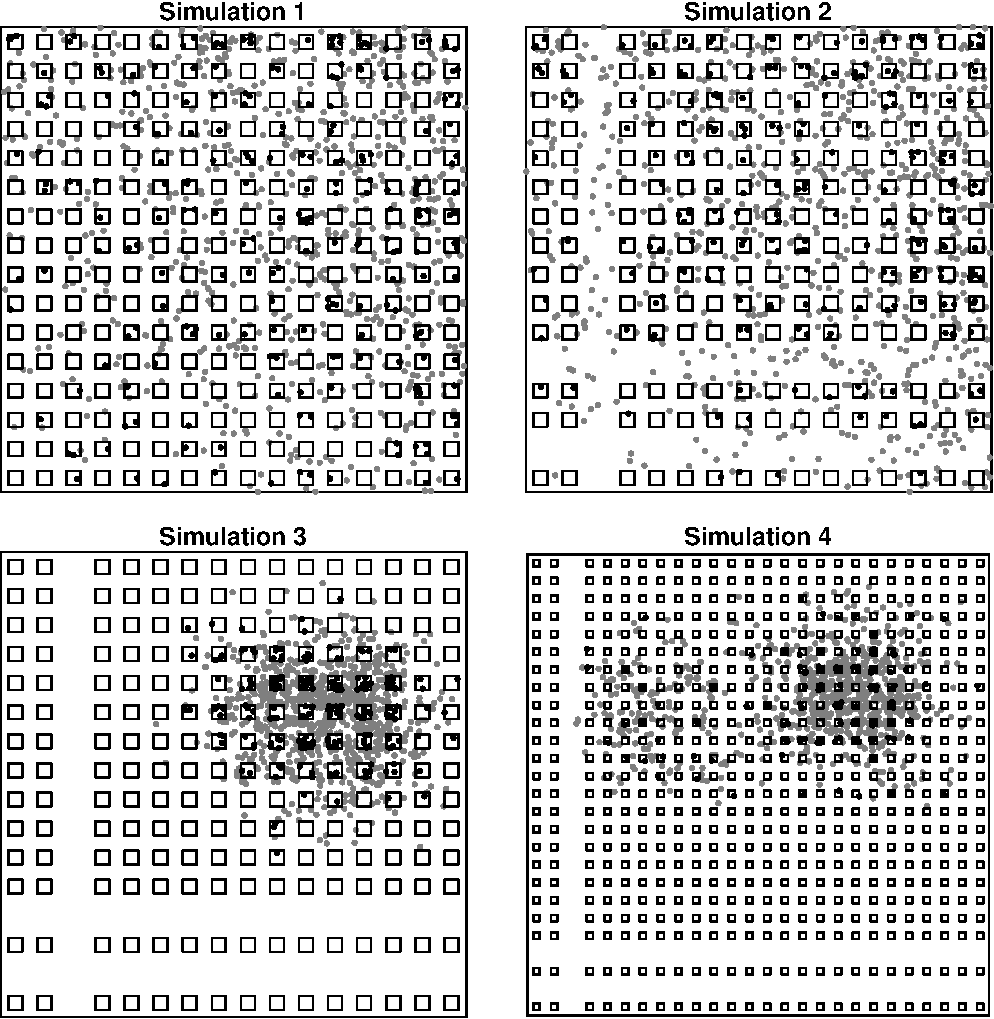
\includegraphics[width = .55\maxwidth]{figure/SimDataCrop}
\end{center}

\end{frame}

%-------------------------------------------------------------------------------
%                        Simulation Experiment 1
%-------------------------------------------------------------------------------

\begin{frame}[fragile]
\frametitle{Simulation Experiment 1}

\footnotesize
\begin{table}[ht]
\centering
\begin{tabular}{rrrrrr}
  \hline
  \hline
	&  & \multicolumn{4}{c}{Knots} \\ 
 & SRS & $\begin{array}{c}K_C=3  \\ K_F=8 \end{array}$ & $\begin{array}{c}K_C=4  \\ K_F=14 \end{array}$ & $\begin{array}{c}K_C=5  \\ K_F=20 \end{array}$ & $\begin{array}{c}K_C=6  \\ K_F=26 \end{array}$ \\
  \hline
bias & 6.425 & -1.277 & -9.735 & 7.048 & 5.941 \\ 
  RMSPE & 58.060 & 57.493 & 59.036 & 58.243 & 58.038 \\ 
  CI90 & 0.914 & 0.898 & 0.883 & 0.892 & 0.895 \\ 
  CI90$_{OD}$ &  & 0.918 & 0.927 & 0.897 & 0.904 \\ 
  CI90$_{WR}$ &  & 0.900 & 0.892 & 0.895 & 0.895 \\ 
  CI90$_{TG}$ &  & 0.914 & 0.920 & 0.939 & 0.957 \\ 
  CI90$_{TL}$ &  & 0.906 & 0.906 & 0.917 & 0.930 \\ 
  fail rate & 0.000 & 0.000 & 0.000 & 0.000 & 0.000 \\ 
   \hline
\end{tabular}
\end{table}

\end{frame}

%-------------------------------------------------------------------------------
%                        Simulation Experiment 2
%-------------------------------------------------------------------------------

\begin{frame}[fragile]
\frametitle{Simulation Experiment 2}

\footnotesize
\begin{table}[ht]
\centering
\begin{tabular}{rrrrrr}
  \hline
  \hline
	&  & \multicolumn{4}{c}{Knots} \\ 
 & SRS & $\begin{array}{c}K_C=3  \\ K_F=8 \end{array}$ & $\begin{array}{c}K_C=4  \\ K_F=14 \end{array}$ & $\begin{array}{c}K_C=5  \\ K_F=20 \end{array}$ & $\begin{array}{c}K_C=6  \\ K_F=26 \end{array}$ \\
  \hline
bias & 79.234 & -1.333 & -7.632 & 14.511 & 13.856 \\ 
  RMSPE & 104.979 & 66.347 & 68.846 & 68.311 & 68.527 \\ 
  CI90 & 0.726 & 0.876 & 0.860 & 0.891 & 0.889 \\ 
  CI90$_{OD}$ &  & 0.908 & 0.928 & 0.901 & 0.902 \\ 
  CI90$_{WR}$ &  & 0.888 & 0.868 & 0.894 & 0.891 \\ 
  CI90$_{TG}$ &  & 0.902 & 0.903 & 0.952 & 0.980 \\ 
  CI90$_{TL}$ &  & 0.895 & 0.880 & 0.927 & 0.940 \\ 
  fail rate & 0.000 & 0.000 & 0.000 & 0.000 & 0.001 \\ 
  \hline
   \hline
\end{tabular}
\end{table}

\end{frame}

%-------------------------------------------------------------------------------
%                        Simulation Experiment 3
%-------------------------------------------------------------------------------

\begin{frame}[fragile]
\frametitle{Simulation Experiment 3}

\footnotesize
\begin{table}[ht]
\centering
\begin{tabular}{rrrrrr}
  \hline
  \hline
	&  & \multicolumn{4}{c}{Knots} \\ 
 & SRS & $\begin{array}{c}K_C=3  \\ K_F=8 \end{array}$ & $\begin{array}{c}K_C=4  \\ K_F=14 \end{array}$ & $\begin{array}{c}K_C=5  \\ K_F=20 \end{array}$ & $\begin{array}{c}K_C=6  \\ K_F=26 \end{array}$ \\
  \hline
bias & 214.816 & -2.389 & -4.365 & -2.919 & -1.637 \\ 
  RMSPE & 235.713 & 79.207 & 79.250 & 79.285 & 80.175 \\ 
  CI90 & 0.774 & 0.775 & 0.772 & 0.781 & 0.777 \\ 
  CI90$_{OD}$ &  & 0.801 & 0.783 & 0.789 & 0.782 \\ 
  CI90$_{WR}$ &  & 0.918 & 0.906 & 0.865 & 0.837 \\ 
  CI90$_{TG}$ &  & 0.923 & 0.930 & 0.929 & 0.946 \\ 
  CI90$_{TL}$ &  & 0.871 & 0.883 & 0.878 & 0.903 \\ 
  fail rate & 0.000 & 0.000 & 0.000 & 0.000 & 0.018 \\ 
   \hline
\end{tabular}
\end{table}

\end{frame}

%-------------------------------------------------------------------------------
%                        Simulation Experiment 4
%-------------------------------------------------------------------------------

\begin{frame}[fragile]
\frametitle{Simulation Experiment 4}

\footnotesize
\begin{table}[ht]
\centering
\begin{tabular}{rrrrrr}
  \hline
  \hline
	&  & \multicolumn{4}{c}{Knots} \\ 
 & SRS & $\begin{array}{c}K_C=3  \\ K_F=8 \end{array}$ & $\begin{array}{c}K_C=5  \\ K_F=16 \end{array}$ & $\begin{array}{c}K_C=7  \\ K_F=24 \end{array}$ & $\begin{array}{c}K_C=9  \\ K_F=32 \end{array}$ \\
  \hline
bias & 148.523 & 5.179 & 3.440 & 7.287 & 14.629 \\ 
  RMSPE & 163.516 & 60.403 & 61.021 & 62.102 & 64.136 \\ 
  CI90 & 0.834 & 0.831 & 0.825 & 0.826 & 0.833 \\ 
  CI90$_{OD}$ &  & 0.844 & 0.831 & 0.827 & 0.833 \\ 
  CI90$_{WR}$ &  & 0.939 & 0.928 & 0.923 & 0.913 \\ 
  CI90$_{TG}$ &  & 0.929 & 0.919 & 0.907 & 0.920 \\ 
  CI90$_{TL}$ &  & 0.893 & 0.892 & 0.884 & 0.886 \\ 
  fail rate & 0.000 & 0.000 & 0.000 & 0.000 & 0.242 \\ 
   \hline
\end{tabular}
\end{table}

\end{frame}

%-------------------------------------------------------------------------------
%                        Simulation Experiment 5
%-------------------------------------------------------------------------------

\begin{frame}[fragile]
\frametitle{Effect of $p$ in Trimmed Overdispersion Estimator}

\begin{center}
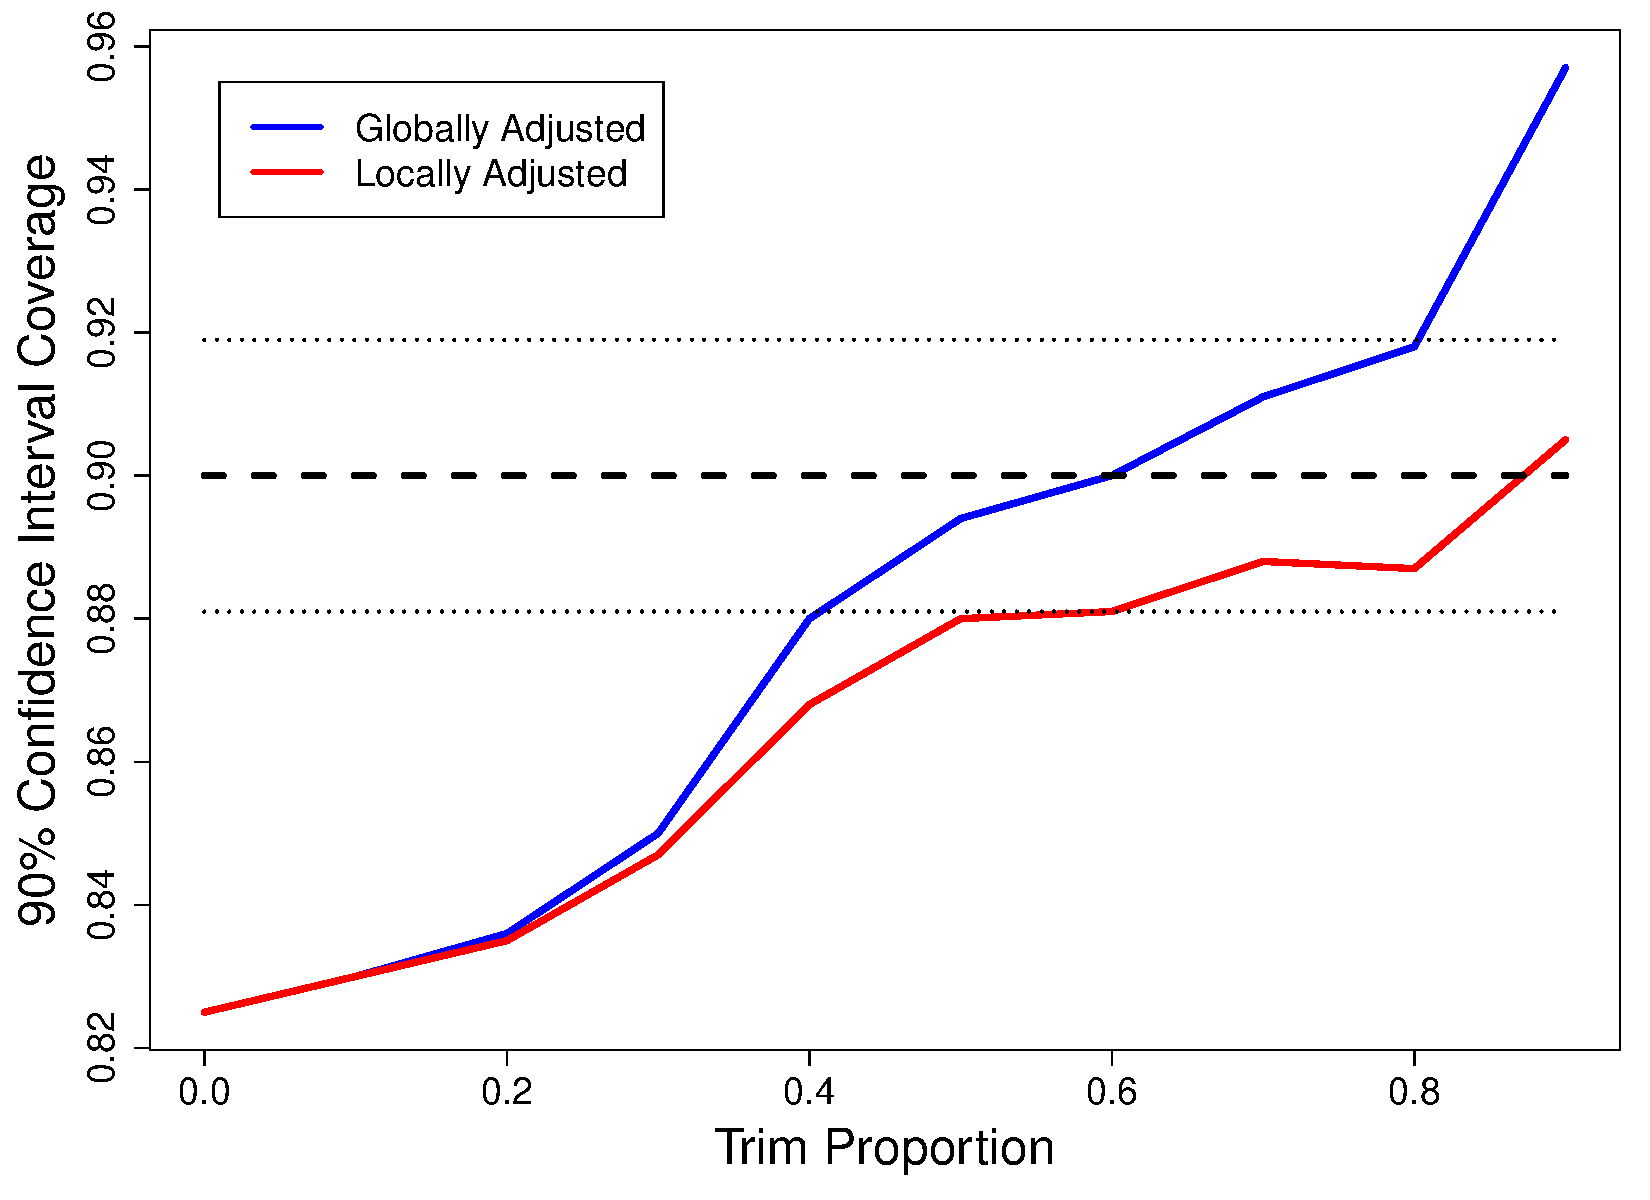
\includegraphics[width = .85\maxwidth]{figure/CI90TrimProp-plot}
\end{center}

\end{frame}

%-------------------------------------------------------------------------------
%                    Real Example
%-------------------------------------------------------------------------------

\section{Example}
\subsection{}
\begin{frame}[fragile]
\frametitle{Real Example}







	\vspace{-.4cm}
	\begin{center}
		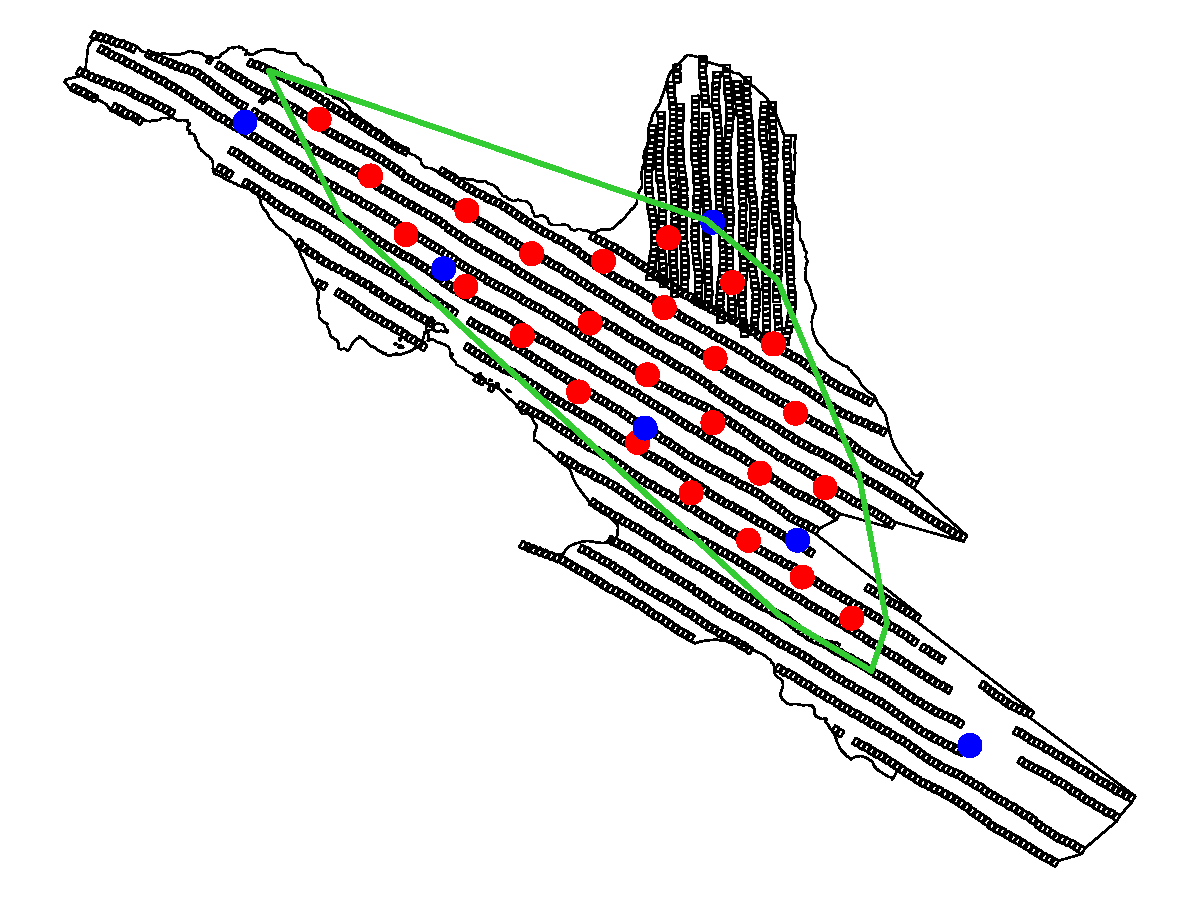
\includegraphics[width = .9\maxwidth]{figure/icyBayKnots-plot}
	\end{center}


\end{frame}

%-------------------------------------------------------------------------------
%                    Real Example
%---------------------------------------------------------]o---------------------

\begin{frame}[fragile]
\frametitle{Real Example}




	\vspace{-.4cm}
	\begin{center}
		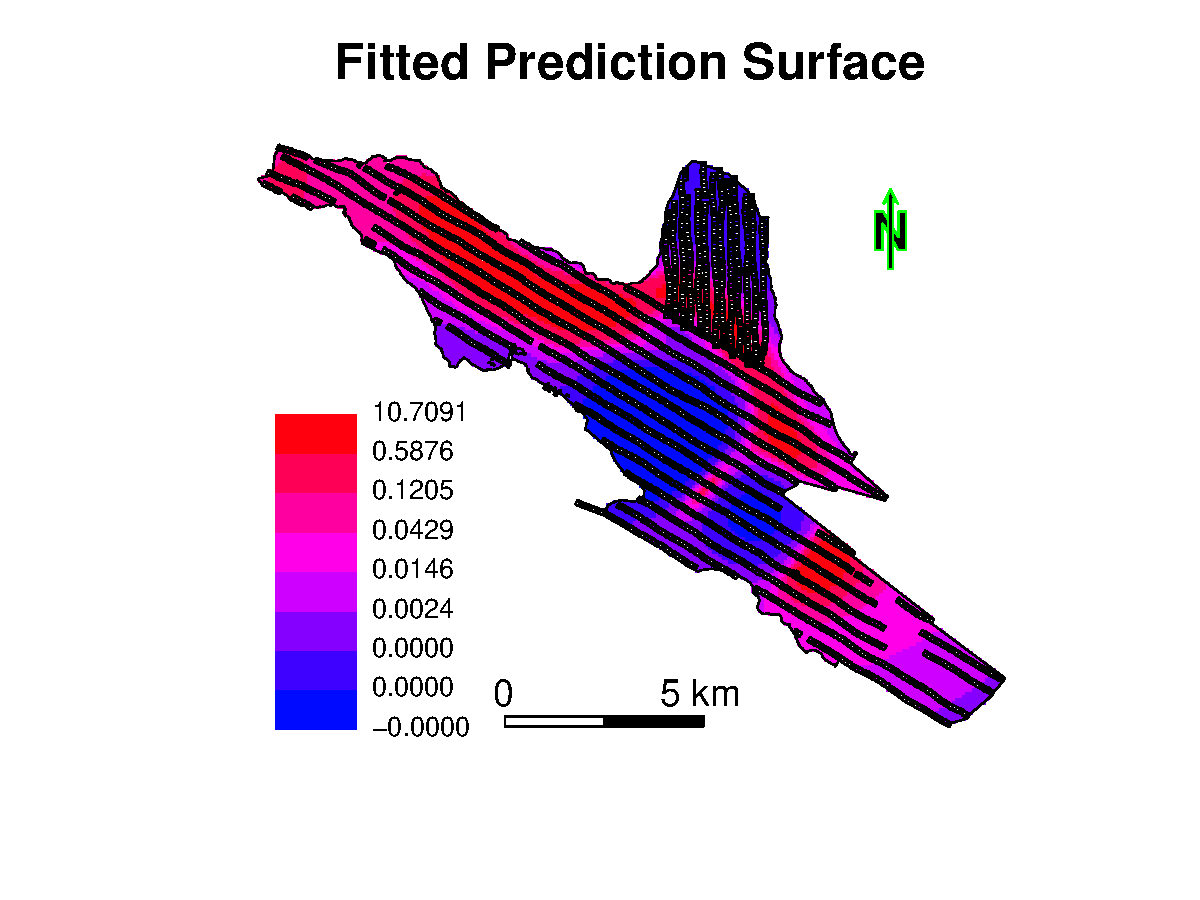
\includegraphics[width = \maxwidth]{figure/icyBayFit-plot}
	\end{center}


\end{frame}

%-------------------------------------------------------------------------------
%                    Real Example
%-------------------------------------------------------------------------------

\begin{frame}[fragile]
\frametitle{Real Example}

\begin{knitrout}\tiny
\definecolor{shadecolor}{rgb}{0.969, 0.969, 0.969}\color{fgcolor}\begin{kframe}
\begin{alltt}
sealDensity <- \hlfunctioncall{sum}(plots@data[, \hlstring{"counts"}])/(sCSout$propSurveyed * totalArea)
sealDensity * totalArea
\end{alltt}
\begin{verbatim}
## [1] 3960
\end{verbatim}
\begin{alltt}
\hlfunctioncall{summary}(sCSout)
\end{alltt}
\begin{verbatim}
## 
## Estimates:
## 
## Total:
## [1] 4068
## Standard Errors:
##      SE SE.ODTrad SE.ODTrimGlobal SE.ODTrimLocal SE.ODRegr
## 1 113.7      1379             236          198.5     403.1
## 
## 
## Range Parameters:
##   coarseScale fineScale
## 1        9516      2974
## 
## 
## Proportion Surveyed:
## [1] 0.253
\end{verbatim}
\end{kframe}
\end{knitrout}


\end{frame}

%-------------------------------------------------------------------------------
%                        Goals
%-------------------------------------------------------------------------------

\section{Summary}
\subsection{}
\begin{frame}[fragile]
\frametitle{Recall the Goals}

\footnotesize
	An estimator that is:
		\begin{itemize}
		\item fast to compute, robust, and requires few modeling decisions, similar to classical survey methods, 			\item based only on counts within plots; actual spatial locations of animals are unknown, 
		\item for the actual number of seals, not the mean of some assumed process that generated the data, 
		\item have a variance estimator with a population correction factor that shrinks to zero as the proportion of the study area that gets sampled goes to one, 
		\item unbiased with valid confidence intervals, 
		\item able to accommodate nonstationary variance and excessive zeros throughout the area
		\end{itemize}

\end{frame}


\end{document}
